\pdfbookmark[0]{Mainbody}{title}
\pagestyle{fancy}
\newgeometry{left=3cm, right=3cm, top=2.79cm, bottom=2cm}
\fancyhead[R]{\textsf{CPT106: User's manual for Car Parking System}}
\fancyhead[L]{}
\fancyfoot[C]{Page \thepage \ of \pageref{LastPage}}
\renewcommand{\headrulewidth}{2pt}
\renewcommand{\baselinestretch}{1.5}
\setcounter{page}{2} 
%\linespread{1.5}
{\rmfamily\selectfont
\vspace{-1ex}
	\section{\textsl{Brief Introduction}}
	{\slshape \selectfont
	\huge	This Car Parking System aims to provide efficient management of parking vehicles in a parking lot. It enables administrators to handle parking spot and customer information, ensures the parking lot doesn't exceed its capacity, supports various types of parking spots, facilitates searching for unoccupied spots, displays available spots on each floor, and implements a per-hour parking fee model for customers.\par
	}
	\newpage
	% 产品的
	\section{product character}
	\subsection{diversity and Searching}
	{\slshape \selectfont
		\huge This system allow administrator and customer to search for all unoccupied parking spots and it support multiple types of parking spots. There are spots for a specific type of vehicle, i.e., car, trunk, van, motorcycle etc.
	}
	\subsection{Fee for parking}
	{\slshape \selectfont\huge
		The system support a per-hour parking fee model. For example, the first hour is free,
		and customers have to pay \$3 for the remaining hours, maximally \$50 per day.
	}
	\subsection{displaying board for free spot}
	{\slshape \selectfont\huge
		Each parking floor has a display board showing any free spot for each spot type. Besides,if the parking is full, the system will show a message to the customer.
	}
	\newpage
	%经理的内容
	\section{For manager}
	\subsection{Searching}
	{\slshape \selectfont\huge
		By entering account,password and floor, managers can easily get each floors information.
		\begin{center}
			\centering
			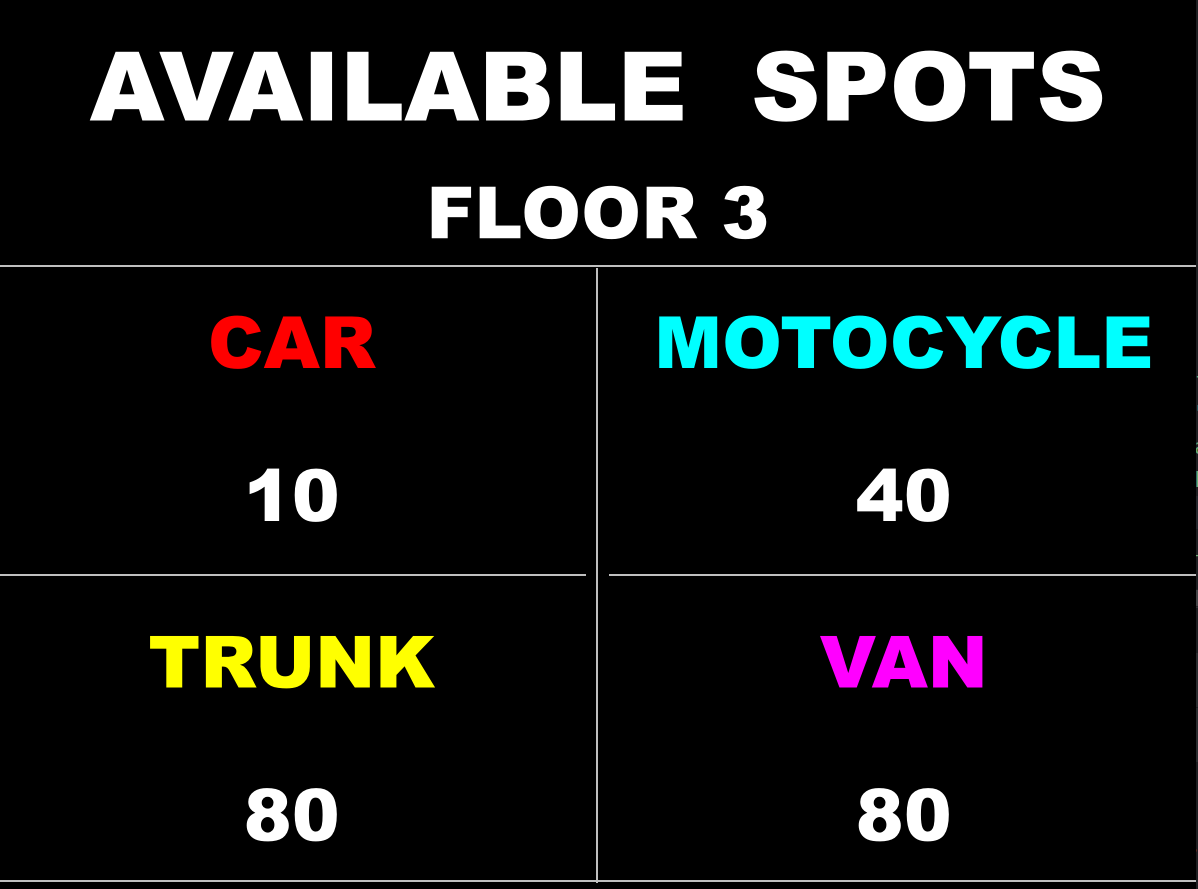
\includegraphics[width=0.4\textwidth]{pics/Floor3.png}
			\captionof{figure}{The informations of each floor}
		\end{center}
	\vspace{10cm}
	\subsection{Tools for editting spot}
	{\slshape \selectfont
	\huge The managers can browse, add, modify and delete spots and customer information
	\begin{center}
	\centering
	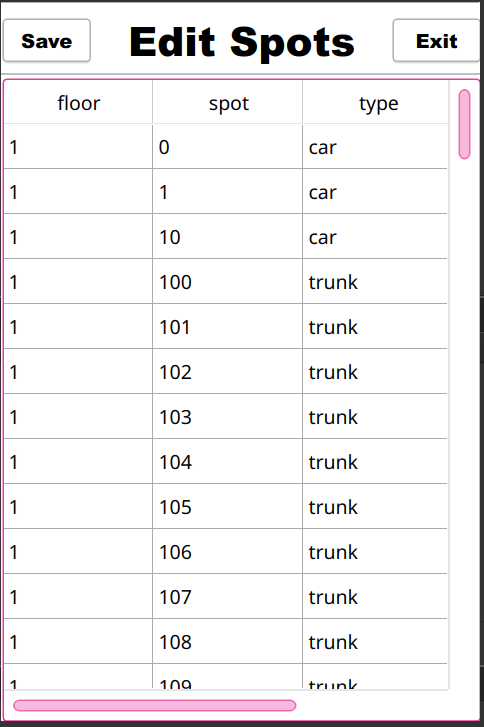
\includegraphics[width=0.4\textwidth]{pics/Edit.png}
	\captionof{figure}{The editor's UI}
	\end{center}
	}
	\newpage
	\section{For customers}
	\subsection{Full Notice}
	{\slshape \selectfont
		\huge Customers will get a notice if the parking is full.
		      And customers can get the information from the display board.
	}
	\subsection{paying}
	{\slshape \selectfont
		\huge When customers enter the park, they can choose the type of vehicle and enter the license plate number.
		\begin{center}
		\centering
		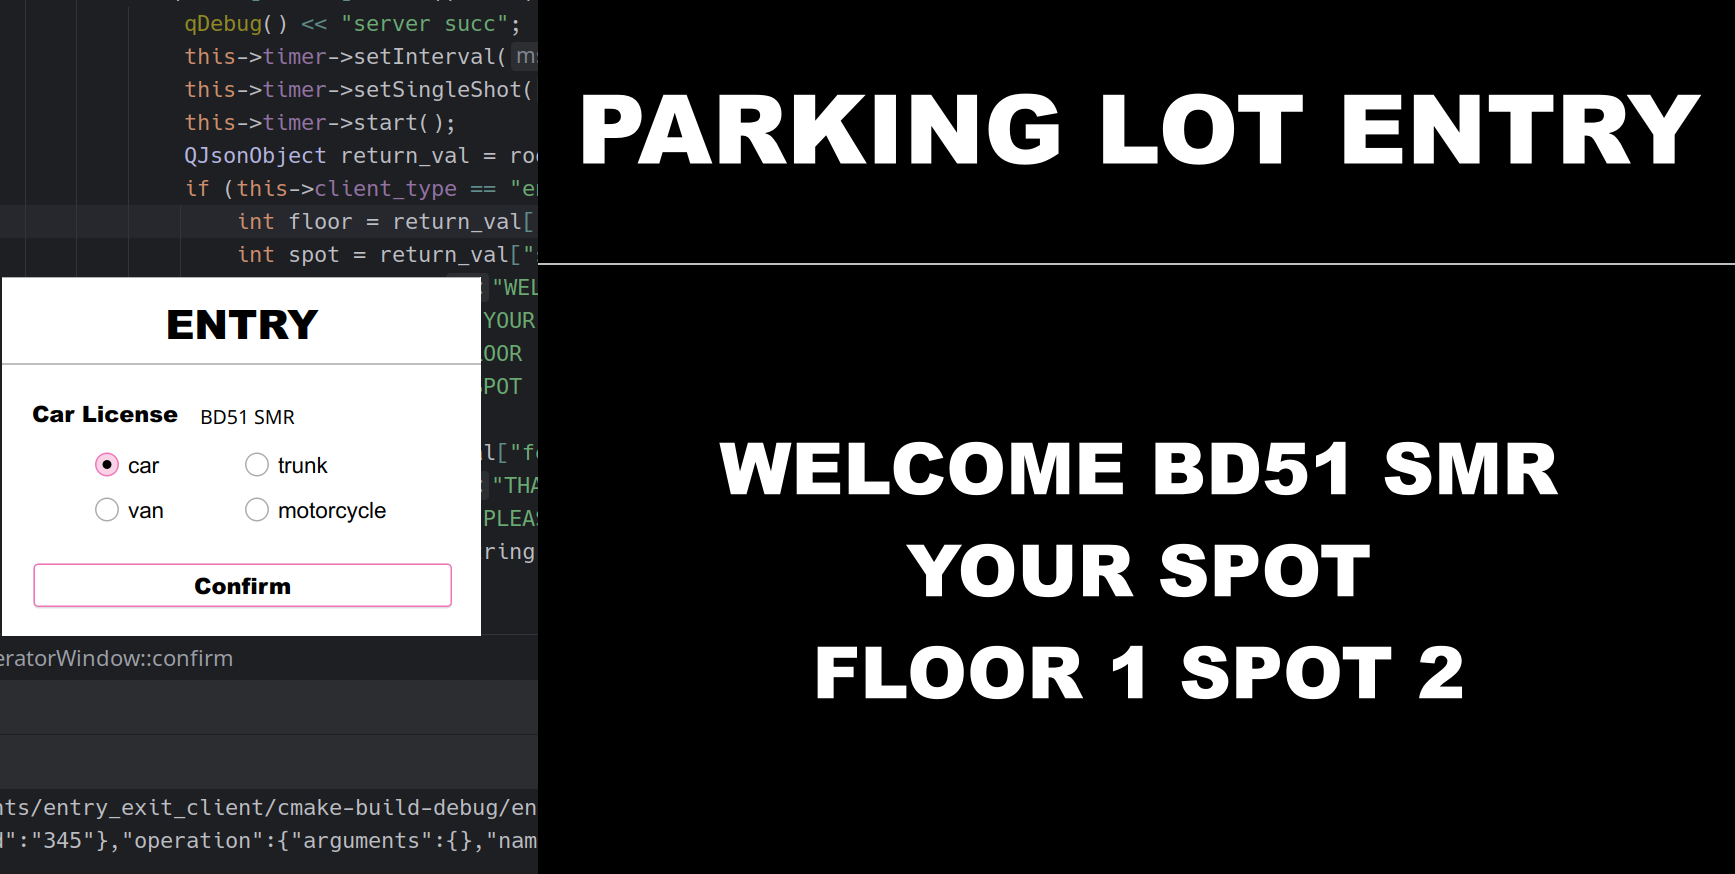
\includegraphics[width=0.8\textwidth]{pics/entry.png}
		\captionof{figure}{The entry UI}
		\end{center}
		\vspace{6cm}
		Then if customers are going to exit the park, this system will calculate the bill and offer port to pay.
		\begin{center}
		\centering
		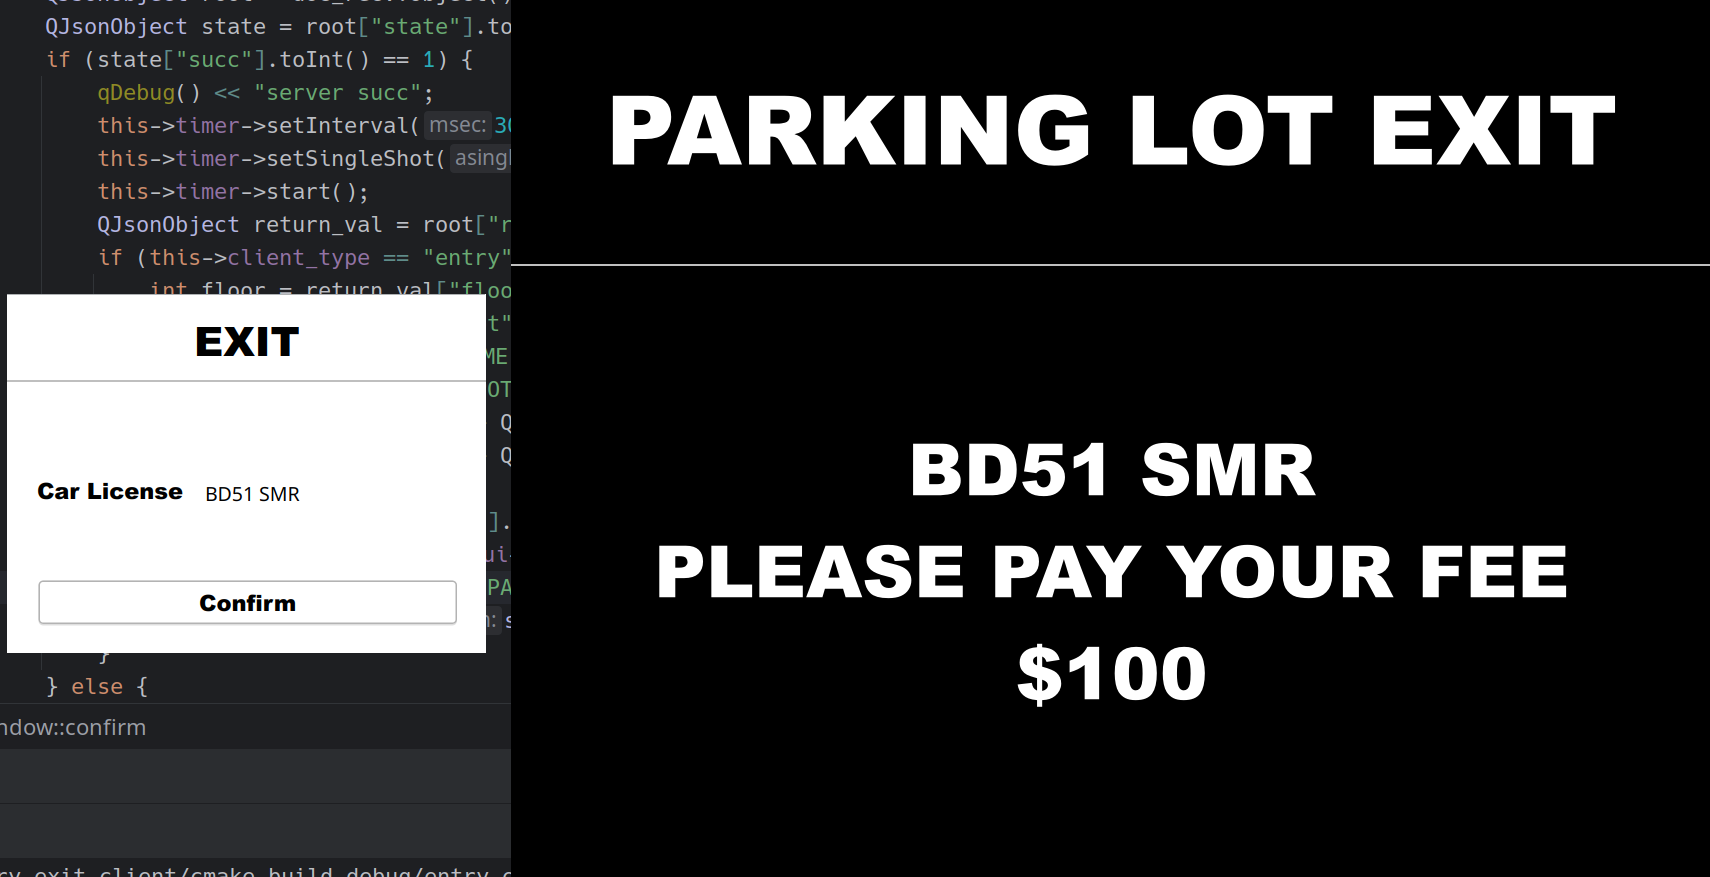
\includegraphics[width=0.6\textwidth]{pics/exit.png}
		\captionof{figure}{The exit UI}
		\end{center}
		
	}
	\subsection{Searching}
	{\slshape \selectfont\huge
		By entering account,password and floor, customers can easily get each floors information.
		\begin{center}
			\centering
			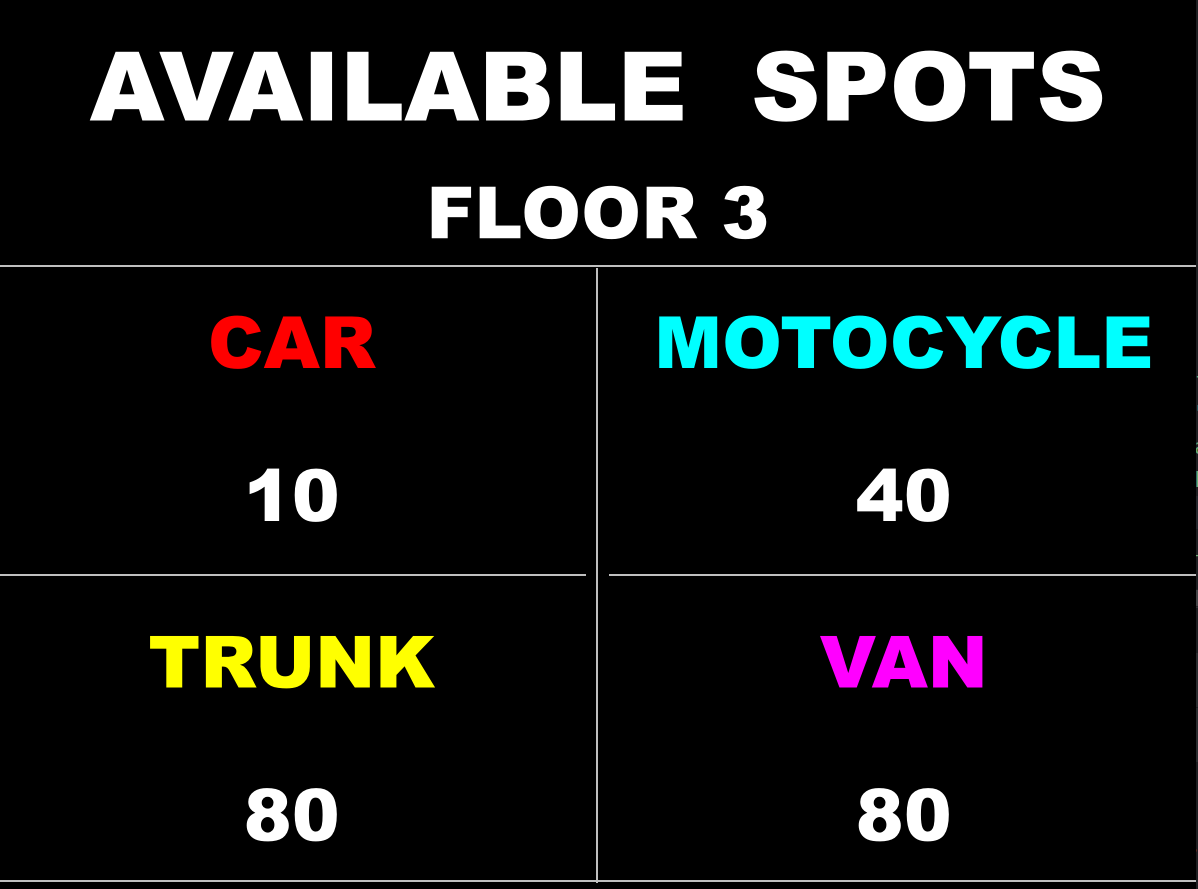
\includegraphics[width=0.4\textwidth]{pics/Floor3.png}
			\captionof{figure}{The informations of each floor}
		\end{center}
	}
}
